\section*{Problema 12.91, Z}


Fluye agua continuamente en un tanque abierto como en la figura. La altura del punto $1$ es de $10m$, y la de los puntos $2$ y $3$ es de $2m$. El área transversal en el punto $2$ es de $0.048m^2$; en el punto $3$ es de $0.016m^2$. El área del tanque es muy grande en comparación con el área transversal del tubo. Suponiendo que puede aplicarse la ecuación de Bernoulli, calcule $a)$ la rapidez de descarga en metros cúbicos por segundo; $b)$ la presión manométrica en el punto $2$.


\begin{figure}[H]
	\centering
	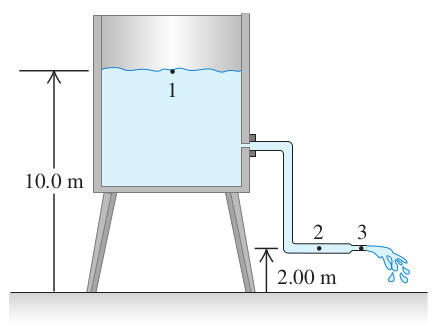
\includegraphics[scale=0.5]{./img/1291.png}
\end{figure}

%%%%